\paragraph{QuizziPedia::Front-End::Views::CreateQuestionnaireView}
\begin{figure} [ht]
	\centering
	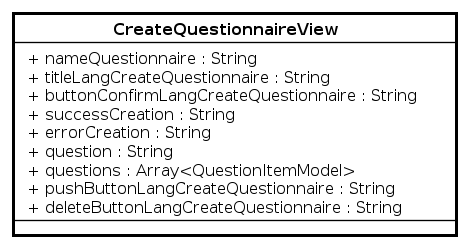
\includegraphics[scale=0.80]{UML/Classi/Front-End/QuizziPedia_Front-end_CreateQuestionnaireView.png}
	\caption{QuizziPedia::Front-End::Views:CreateQuestionnaireView}
\end{figure} \FloatBarrier
\begin{itemize}
	\item \textbf{Descrizione}: \textit{view\ped{G}} per la creazione del questionario. In questo componente viene permesso anche all'utente di:
	\begin{itemize}
		\item Effettuare delle ricerche sul database di domande;
		\item Selezionare le domande da inserire nel questionario;
		\item Mostrare le domande già inserite e permettere all'utente di eliminarle da tale lista.
	\end{itemize}
	\item \textbf{Utilizzo}: permette all'utente di creare un questionario compilando tutti i campi proposti;
	\item \textbf{Relazioni con altre classi}:
	\begin{itemize}
		\item \textbf{IN \texttt{CreateQuestionnaireModelView}}: classe di tipo modelview la cui istanziazione è contenuta all'interno della variabile di ambiente \texttt{\$scope} di \textit{Angular\ped{G}}. All'interno di essa sono presenti le variabili e i metodi necessari per il \textit{Two-Way Data-Binding\ped{G}} tra la \textit{view\ped{G}} \texttt{CreateQuestionnaireView} e il \textit{controller\ped{G}} \texttt{CreateQuestionnaireController};
		\item \textbf{IN \texttt{TopicKeywordsDirective}}: \textit{directive\ped{G}} che permette di gestire l'inserimento dell'argomento e delle keywords al momento della creazione della domanda;
		\item \textbf{IN \texttt{LangModel}}: rappresenta il modello delle informazioni per la giusta traduzione dell'applicazione.
	\end{itemize}
		\item \textbf{Attributi}:
		\begin{itemize}
			\item \texttt{+ nameQuestionnaire: String}: \\ Attributo che specifica il nome del questionario creato;
			\item \texttt{+ titleLangCreateQuestionnaire: String} \\ Attributo che viene utilizzato per visualizzare la giusta traduzione del titolo della pagina, in italiano o in inglese;
			\item \texttt{+ buttonConfirmLangCreateQuestionnaire: String} \\ Attributo che viene utilizzato per visualizzare la giusta traduzione della \textit{label\ped{G}} per il bottone di conferma, in italiano o in inglese;
			\item \texttt{+ successCreation: String} \\ Attributo che visualizza un messaggio di conferma avvenuta creazione della domanda;
			\item \texttt{+ errorCreation: String} \\ Attributo che visualizza un messaggio d'errore per la creazione della domanda.
			\item \texttt{+ question: String} \\ Attributo che conterrà la stringa per la ricerca della domanda;
			\item \texttt{+ questions: Array<QuestionItemModel>} \\ \texttt{array} contenente le domande trovate durante la ricerca;
			\item \texttt{+ pushButtonLangCreateQuestionnaire: String} \\ Attributo che viene utilizzato per visualizzare la giusta traduzione della \textit{label\ped{G}} per il bottone di inserimento delle domande selezionate, in italiano o in inglese;
			\item \texttt{+ deleteButtonLangCreateQuestionnaire: String} \\ Attributo che viene utilizzato per visualizzare la giusta traduzione della \textit{label\ped{G}} per il bottone di eliminazione delle domande dal questionario, in italiano o in inglese.
		\end{itemize}
\end{itemize}